\section{Series of Real Numbers} \label{S:8.3.Series}

\vspace*{-14 pt}
\framebox{\hspace*{3 pt}
\parbox{\boxwidth}{\begin{goals}
\item What is an infinite series?
\item What is the $n$th partial sum of an infinite series?
\item How do we add up an infinite number of numbers? In other words, what does it mean for an infinite series of real numbers to converge?
\item What does is mean for an infinite series of real numbers to diverge?
\end{goals}} \hspace*{3 pt}}

\subsection*{Introduction}

In Section~\ref{S:8.2.Geometric}, we encountered several situations where we naturally considered an infinite sum of numbers called a geometric series.  For example, by writing
$$N = 0.1212121212 \cdots = \frac{12}{100} + \frac{12}{100} \cdot \frac{1}{100} + \frac{12}{100} \cdot \frac{1}{100^2} + \cdots$$
as a geometric series, we found a way to write the repeating decimal expansion of $N$ as a single fraction: $N = \frac{4}{33}$.  There are many other situations in mathematics where infinite sums of numbers arise, but often these are not geometric.  In this section, we begin exploring these other types of infinite sums.  Preview Activity~\ref{PA:8.3} provides a context in which we see how one such sum is related to the famous number $e$.

\begin{pa} \label{PA:8.3}
Have you ever wondered how your calculator can produce a numeric approximation for complicated numbers like $e$, $\pi$ or $\ln(2)$? After all, the only operations a calculator can really perform are addition, subtraction, multiplication, and division, the operations that make up polynomials. This activity provides the first steps in understanding how this process works. Throughout the activity, let $f(x) = e^x$.

\ba
\item Find the tangent line to $f$ at $x=0$ and use this linearization to approximate $e$.  That is, find a formula $L(x)$ for the tangent line, and compute $L(1)$, since $L(1) \approx f(1) = e$.

\begin{activitySolution}

The linearization of $f$ at $x=a$ is
\[f(a) + f'(a)(x-a),\]
so the linearization $P_1(x)$ of $f(x) = e^x$ at $x=0$ is
\[P_1(x) = e^0 + e^0(x-0) = 1+x.\]
Now
\[f(x) \approx P_1(x)\]
for $x$ close to $0$ and so
\[e = e^1 \approx P_1(1) = 1+1 = 2.\]

\end{activitySolution}

\item The linearization of $e^x$ does not provide a good approximation to $e$ since 1 is not very close to 0. To obtain a better approximation, we alter our approach a bit. Instead of using a straight line to approximate $e$, we put an appropriate bend in our estimating function to make it better fit the graph of $e^x$ for $x$ close to 0. With the linearization, we had both $f(x)$ and $f'(x)$ share the same value as the linearization at $x=0$. We will now use a quadratic approximation $P_2(x)$ to $f(x) = e^x$ centered at $x=0$ which has the property that $P_2(0) = f(0)$, $P'_2(0) = f'(0)$, \text{and} $P''_2(0) = f''(0)$.

     \begin{itemize}
     \item[(i)] Let $P_2(x) = 1+x+\frac{x^2}{2}$. Show that $P_2(0) = f(0)$, $P'_2(0) = f'(0)$, and $P''_2(0) = f''(0)$. Then, use $P_2(x)$ to approximate $e$ by observing that $P_2(1) \approx f(1)$.

\begin{activitySolution}

The derivatives of $P_2$ and $f$ are
\begin{align*}
P_2(x) &= 1+x+\frac{x^2}{2} & f(x) &= e^x \\
P'_2(x) &= 1 + x & f'(x) &= e^x \\
P''_2(x) &= 1 & f''(x) &= e^x,
\end{align*}
and so the derivatives of $P_2$ and $f$ evaluated at 0 are
\begin{align*}
P_2(0) &= 1 & f(0) &= e^0 = 1 \\
P'_2(0) &= 1 & f'(0) &= e^0 = 1 \\
P''_2(0) &= 1 & f''(0) &= e^0 = 1.
\end{align*}
Then
\[e = e^1 \approx P_2(1) = 1 + 1 + \frac{1}{2} = 2.5.\]

\end{activitySolution}

    \item[(ii)] We can continue approximating $e$ with polynomials of larger degree whose higher derivatives agree with those of $f$ at 0. This turns out to make the polynomials fit the graph of $f$ better for more values of $x$ around 0. For example, let $P_3(x) = 1+x+\frac{x^2}{2}+\frac{x^3}{6}$. Show that $P_3(0) = f(0)$, $P'_3(0) = f'(0)$, $P''_3(0) = f''(0)$, and $P'''_3(0) = f'''(0)$. Use $P_3(x)$ to approximate $e$ in a way similar to how you did so with $P_2(x)$ above.

\begin{activitySolution}

The derivatives of $P_3$ and $f$ are
\begin{align*}
P_3(x) &= 1+x+\frac{x^2}{2}+\frac{x^3}{6} & f(x) &= e^x \\
P'_3(x) &= 1 + x +\frac{x^2}{2}  & f'(x) &= e^x \\
P''_3(x) &= 1+x  & f''(x) &= e^x \\
P'''_3(x) &= 1  & f'''(x) &= e^x,
\end{align*}
and so the derivatives of $P_2$ and $f$ evaluated at 0 are
\begin{align*}
P_3(0) &= 1 & f(0) &= e^0 = 1 \\
P'_3(0) &= 1 & f'(0) &= e^0 = 1 \\
P''_3(0) &= 1 & f''(0) &= e^0 = 1 \\
P'''_3(0) &= 1 & f'''(0) &= e^0 = 1.
\end{align*}
Then
\[e = e^1 \approx P_3(1) = 1 + 1 + \frac{1}{2} + \frac{1}{6} = \frac{8}{3} \approx 2.67.\]

\end{activitySolution}
        
    \end{itemize}
  \ea

\end{pa}
\afterpa 

Preview Activity \ref{PA:8.3} shows that an approximation to $e$ using a linear polynomial is 2, an approximation to $e$ using a quadratic polynomial is $2.5$, and an approximation using a cubic polynomial is 2.6667. As we will see later, if we continue this process we can obtain approximations from quartic (degree 4), quintic (degree 5), and higher degree polynomials giving us the following approximations to $e$:
\begin{center}
\renewcommand{\arraystretch}{1.5}
\begin{tabular}{lll} \hline
linear  &$1 + 1$              & $2$ \\ \hline
quadratic &$1 +1 + \frac{1}{2}$     & $2.5$ \\ \hline
cubic &$1 + 1 + \frac{1}{2} + \frac{1}{6}$      &$2.\overline{6}$ \\ \hline
quartic  &$1 + 1 +  \frac{1}{2} + \frac{1}{6} + \frac{1}{24}$   & $2.708\overline{3}$ \\ \hline
quintic  &$1 + 1 + \frac{1}{2} + \frac{1}{6} + \frac{1}{24} + \frac{1}{120}$    & $2.71\overline{6}$ \\ \hline
\end{tabular}
\end{center}
We see an interesting pattern here. The number $e$ is being approximated by the sum
\begin{equation} \label{eq:8.3_e_n}
1+1+\frac{1}{2} + \frac{1}{6} + \frac{1}{24} + \frac{1}{120} + \cdots + \frac{1}{n!}
\end{equation}
for increasing values of $n$.
And just as we did with Riemann sums, we can use the summation notation as a shorthand\footnote{Note that $0!$ appears in Equation~(\ref{eq:8.3_e}).  By definition, $0! = 1$.} for writing the sum in Equation~(\ref{eq:8.3_e_n}) so that
\begin{equation} \label{eq:8.3_e}
e \approx 1+1+\frac{1}{2} + \frac{1}{6} + \frac{1}{24} + \frac{1}{120} + \cdots + \frac{1}{n!} = \sum_{k=0}^n \frac{1}{k!}.
\end{equation}
We can calculate this sum using as large an $n$ as we want, and the larger $n$ is the more accurate the approximation (\ref{eq:8.3_e}) is. Ultimately, this argument shows that we can write the number $e$ as the infinite sum
\begin{equation} \label{eq:8.3_e_infinite}
e = \sum_{k=0}^{\infty} \frac{1}{k!}.
\end{equation}
This sum is an example of a \emph{series}\index{series} (or an \emph{infinite series}\index{infinite series}). Note that the series~(\ref{eq:8.3_e_infinite}) is the sum of the terms of the (infinite) sequence $\left\{\frac{1}{n!}\right\}$.  In general, we use the following notation and terminology.

\begin{definition} An \emph{infinite series} of real numbers is the sum of the entries in an infinite sequence of real numbers. In other words, an infinite series is sum of the form
 \[a_1+a_2+ \cdots + a_n + \cdots = \sum_{k=1}^{\infty} a_k,\]
where $a_1$, $a_2$, $\ldots$, are real numbers. 
\end{definition}

We will normally use summation notation to identify a series. If the series adds the entries of a sequence $\{a_n\}_{n \geq 1}$, then we will write the series as
\[\sum_{k \geq 1} a_k\]
or
\[\sum_{k=1}^{\infty} a_k.\]
Note well: each of these notations is simply shorthand for the infinite sum $a_1 + a_2 + \cdots + a_n + \cdots$.

Is it even possible to sum an infinite list of numbers?  This question is one whose answer shouldn't come as a surprise. After all, we have used the definite integral to add up continuous (infinite) collections of numbers, so summing the entries of a sequence might be even easier.  Moreover, we have already examined the special case of geometric series in the previous section. The next activity provides some more insight into how we make sense of the process of summing an infinite list of numbers.

\begin{activity} \label{8.3.Act1} Consider the series
\[\sum_{k=1}^{\infty} \frac{1}{k^2}.\]
While it is physically impossible to add an infinite collection of numbers, we can, of course, add any finite collection of them.  In what follows, we investigate how understanding how to find the $n$th partial sum (that is, the sum of the first $n$ terms) enables us to make sense of the infinite sum.
\ba
\item Sum the first two numbers in this series. That is, find a numeric value for
\[\sum_{k=1}^2 \frac{1}{k^2}\]

\item Next, add the first three numbers in the series.

\item Continue adding terms in this series to complete Table~\ref{T:8.3.1_part_sum_ex}. Carry each sum to at least 8 decimal places.
\begin{table}[ht]
\begin{center}
\renewcommand{\arraystretch}{1.5}
\begin{tabular}{r c p{0.5in} p{1.0in} r c p{0.5in}}
$\ds \sum_{k=1}^{1} \frac{1}{k^2}$   & = & $1$  &   &$\ds \sum_{k=1}^{6} \frac{1}{k^2}$   &= & \\
$\ds \sum_{k=1}^{2} \frac{1}{k^2}$   & = &     &   &$\ds \sum_{k=1}^{7} \frac{1}{k^2}$   & = & \\
$\ds \sum_{k=1}^{3} \frac{1}{k^2}$   & = &     &   &$\ds \sum_{k=1}^{8} \frac{1}{k^2}$   & = &  \\
$\ds \sum_{k=1}^{4} \frac{1}{k^2}$   & = &     &   &$\ds \sum_{k=1}^{9} \frac{1}{k^2}$   &  = &\\
$\ds \sum_{k=1}^{5} \frac{1}{k^2}$   & = &     &   &$\ds \sum_{k=1}^{10} \frac{1}{k^2}$  & = & \\
\end{tabular}
\caption{Sums of some of the first terms of the series $\sum_{k=1}^{\infty} \frac{1}{k^2}$} \label{T:8.3.1_part_sum_ex}
\end{center}
\end{table}

\item The sums in the table in (c) form a sequence whose $n$th term is $S_n =  \sum_{k=1}^{n} \frac{1}{k^2}$. Based on your calculations in the table, do you think the sequence $\{S_n\}$ converges or diverges? Explain. How do you think this sequence $\{S_n\}$ is related to the series $ \sum_{k=1}^{\infty} \frac{1}{k^2}$?

\ea
\end{activity}

\begin{smallhint}
\ba
	\item Small hints for each of the prompts above.
\ea
\end{smallhint}
\begin{bighint}
\ba
	\item Big hints for each of the prompts above.
\ea
\end{bighint}
\begin{activitySolution}
\ba
	\item See the Table in part (c).
    \item See the Table in part (c).
    \item If we add the first few terms of the sequence $\left\{\frac{1}{k^2}\right\}$ we obtain the entries (to 10 decimal places) in the following table.
%\begin{table}[ht]
\begin{center}
\renewcommand{\arraystretch}{1.5}
\begin{tabular}{c|c p{1.0in} c|c}
$\ds \sum_{k=1}^{1} \frac{1}{k^2}$   & $1$              &   &$\ds \sum_{k=1}^{6} \frac{1}{k^2}$   & $1.491388889$ \\
$\ds \sum_{k=1}^{2} \frac{1}{k^2}$   & $1.25$           &   &$\ds \sum_{k=1}^{7} \frac{1}{k^2}$   & $1.511797052$ \\
$\ds \sum_{k=1}^{3} \frac{1}{k^2}$   & $1.361111111$    &   &$\ds \sum_{k=1}^{8} \frac{1}{k^2}$   & $1.527422052$ \\
$\ds \sum_{k=1}^{4} \frac{1}{k^2}$   & $1.423611111$    &   &$\ds \sum_{k=1}^{9} \frac{1}{k^2}$   & $1.539767731$ \\
$\ds \sum_{k=1}^{5} \frac{1}{k^2}$   & $1.463611111$    &   &$\ds \sum_{k=1}^{10} \frac{1}{k^2}$  & $1.549767731$ \\
\end{tabular}
%\label{T:8.3.1_part_sum_ex_b}
%\caption{Sums of some of the first terms of the series $\sum_{k=1}^{\infty} \frac{1}{k^2}$}
\end{center}
%\end{table}
    \item These sums in the table in part (c) seem to indicate that the sequence $\{S_n\}$ converges to something a bit larger than 1.5. Since the sequence $\{S_n\}$ is found by adding up the first $k$ terms of the series, we should expect that the series $\ds \sum_{k=1}^{n} \frac{1}{k^2}$ is the limit of the sequence $\{S_n\}$ as $n$ goes to infinity.
\ea
\end{activitySolution}
\aftera 

The example in Activity \ref{8.3.Act1} illustrates how we define the sum of an infinite series. We can add up the first $n$ terms of the series to obtain a new sequence of numbers (called the \emph{sequence of partial sums}\index{partial sum}\index{sequence of partial sums}). Provided that sequence converges, the corresponding infinite series is said to converge, and we say that we can find the sum of the series.

\begin{definition} The \emph{$n$th partial sum} of the series $\sum_{k=1}^{\infty} a_k$
is the finite sum
$S_n = \sum_{k=1}^{n} a_k.$
\end{definition}
In other words, the $n$th partial sum $S_n$ of a series is the sum of the first $n$ terms in the series, or
\[S_n = a_1 + a_2 + \cdots + a_n.\]
We then investigate the behavior of a given series by examining the sequence
\[S_1, S_2, \ldots, S_n, \ldots\]
of its partial sums.  If the sequence of partial sums converges to some finite number, then we say that the corresponding series \emph{converges}\index{series!converges}. Otherwise, we say the series \emph{diverges}\index{series!diverges}. From our work in Activity~\ref{8.3.Act1}, the series
\[\sum_{k=1}^{\infty} \frac{1}{k^2}\]
appears to converge to some number near 1.54977.  We formalize the concept of convergence and divergence of an infinite series in the following definition.

\begin{definition} The infinite series
\[\sum_{k=1}^{\infty} a_k\]
\emph{converges} (or is \emph{convergent}) if the sequence $\{S_n\}$ of partial sums converges, where
\[S_n = \sum_{k=1}^n a_k.\]
If $\lim_{n \to \infty} S_n = S$, then we call $S$ the sum of the series $\sum_{k=1}^{\infty} a_k$.  That is,
\[\sum_{k=1}^{\infty} a_k = \lim_{n \to \infty} S_n = S.\]
If the sequence of partial sums does not converge, then the series
\[\sum_{k=1}^{\infty} a_k\]
\emph{diverges} (or is \emph{divergent}).
\end{definition}

The early terms in a series do not contribute to whether or not the series converges or diverges. Rather, the convergence or divergence of a series
\[\sum_{k=1}^{\infty} a_k\]
is determined by what happens to the terms $a_k$ for very large values of $k$. To see why, suppose that  $m$ is some constant larger than 1.  Then
\[\sum_{k=1}^{\infty} a_k = (a_1+a_2+ \cdots + a_m) + \sum_{k=m+1}^{\infty} a_k.\]
Since $a_1+a_2+ \cdots + a_m$ is a finite number, the series $\sum_{k=1}^{\infty} a_k$ will converge if and only if the series $\sum_{k=m+1}^{\infty} a_k$ converges. Because the starting index of the series doesn't affect whether the series converges or diverges, we will often just write
\[\sum a_k\]
when we are interested in questions of convergence/divergence and not necessarily the exact sum of a series.

In Section~\ref{S:8.2.Geometric} we encountered the special family of infinite geometric series whose convergence or divergence we completely determined. Recall that a geometric series is a special series of the form $\sum_{k=0}^{\infty} ar^k$ where $a$ and $r$ are real numbers (and $r \ne 1$). We found that the $n$th partial sum $S_n$ of a geometric series is given by the convenient formula 
$$S_n = \frac{1-r^{n}}{1-r},$$ 
and thus a geometric series converges if $|r| < 1$.  Geometric series diverge for all other values of $r$. While we have completely determined the convergence or divergence of geometric series, it is generally a difficult question to determine if a given nongeometric series converges or diverges. There are several tests we can use that we will consider in the following sections.

\subsection*{The Divergence Test}
The first question we ask about any infinite series is usually ``Does the series converge or diverge?''  There is a straightforward way to check that certain series diverge; we explore this test in the next activity.

\begin{activity} \label{8.3.Act2} If the \emph{series} $\sum a_k$ converges, then an important result necessarily follows regarding the \emph{sequence} $\{a_n\}$. This activity explores this result. 

Assume that the series $ \sum_{k=1}^{\infty} a_k$ 
converges and has sum equal to $L$. 

\ba
\item What is the $n$th partial sum $S_n$ of the series $ \sum_{k=1}^{\infty} a_k$?

\item What is the $(n-1)$st partial sum $S_{n-1}$ of the series $ \sum_{k=1}^{\infty} a_k$?

\item What is the difference between the $n$th partial sum and the $(n-1)$st partial sum of the series $ \sum_{k=1}^{\infty} a_k$?

\item Since we are assuming that  $ \sum_{k=1}^{\infty} a_k = L$, what does that tell us about $ \lim_{n \to \infty} S_n$? Why?  What does that tell us about $ \lim_{n \to \infty} S_{n-1}$? Why?



\item Combine the results of the previous two parts of this activity to determine $ \lim_{n \to \infty} a_n = \lim_{n \to \infty} (S_n - S_{n-1})$.


\ea

\end{activity}

\begin{smallhint}
\ba
	\item Small hints for each of the prompts above.
\ea
\end{smallhint}
\begin{bighint}
\ba
	\item Big hints for each of the prompts above.
\ea
\end{bighint}
\begin{activitySolution}
\ba
	\item The $n$th partial sum of the series $\ds \sum_{k=1}^{\infty} a_k$ is
\[S_n = \sum_{k=1}^n a_k.\]
    \item The $(n-1)$st partial sum of the series $\ds \sum_{k=1}^{\infty} a_k$ is
\[S_{n-1} = \sum_{k=1}^{n-1} a_k.\]
    \item The difference between $S_n$ and $S_{n-1}$ is
\[\sum_{k=1}^{n} a_k - \sum_{k=1}^{n-1} a_k = a_{n}.\]
    \item Since  $\ds \sum_{k=1}^{\infty} a_k = \lim_{n \to \infty} S_n$ we must have $\lim_{n \to \infty} S_n = L$. Also,
\[\lim_{n \to \infty} S_n = \lim_{n \to \infty} S_{n-1},\]
so $\lim_{n \to \infty} S_{n-1} = L$ as well.
    \item We have
\begin{align*}
\lim_{n \to \infty} a_n &= \lim_{n \to \infty} \left(S_n - S_{n-1}\right) \\
    &= \lim_{n \to \infty} S_n - \lim_{n \to \infty} S_{n-1} \\
    &= L - L \\
    &= 0.
\end{align*}

\ea
\end{activitySolution}
\aftera 

The result of Activity \ref{8.3.Act2} is the following important conditional statement: 
\begin{quote}
If the series $\ds \sum_{k = 1}^{\infty} a_k$ converges, then the sequence $\{a_k\}$ of $k$th terms converges to 0.
\end{quote}
It is logically equivalent to say that if the sequence $\{a_k\}$ of $n$ terms does not converge to 0, then the series $ \sum_{k = 1}^{\infty} a_k$ cannot converge. This statement is called the Divergence Test\index{Divergence Test}.

\vspace*{5pt}
\nin \framebox{\hspace*{3 pt}
\parbox{\boxwidth}{
\textbf{The Divergence Test. } If $\lim_{k \to \infty} a_k \neq 0$, then the series $\ds \sum a_k$
diverges.
} \hspace*{3 pt}}
\vspace*{1pt}

\begin{activity} \label{8.3.Act3} Determine if the Divergence Test applies to the following series. If the test does not apply, explain why. If the test does apply, what does it tell us about the series?

\ba
\item  $\sum \frac{k}{k+1}$
\item  $\sum (-1)^k $

\item  $\sum \frac{1}{k}$

\ea
\end{activity}

\begin{smallhint}
\ba
	\item Small hints for each of the prompts above.
\ea
\end{smallhint}
\begin{bighint}
\ba
	\item Big hints for each of the prompts above.
\ea
\end{bighint}
\begin{activitySolution}
\ba
	\item Since the sequence $\frac{k}{k+1}$ converges to 1 and not 0 as $k$ goes to infinity, the Divergence Test applies here and shows that the series $\sum \frac{k}{k+1}$ diverges.
    \item Since $\ds \lim_{k \to \infty} \frac{1}{k} = 0$, the Divergence Test does not apply to this series. 
\ea
\end{activitySolution}
\aftera 


{\bf Note well:} be very careful with the Divergence Test. This test only tells us what happens to a series if the terms of the corresponding sequence do not converge to 0. If the sequence of the terms  of the series does converge to 0, the Divergence Test does not apply:  indeed, as we will soon see, a series whose terms go to zero may either converge or diverge.

\subsection*{The Integral Test}\index{integral test}

The Divergence Test settles the questions of divergence or convergence of series $\sum a_k$ in which $\lim_{k \to \infty} a_k \neq 0$.  Determining the convergence or divergence of series $\sum a_k$ in which $\lim_{k \to \infty} a_k = 0$ turns out to be more complicated. Often, we have to investigate the sequence of partial sums or apply some other technique.

As an example, consider the \emph{harmonic}\index{harmonic series} series\footnote{This series is called harmonic because each term in the series after the first is the harmonic mean of the term  before it and the term after it. The harmonic mean of two numbers $a$ and $b$ is $\frac{2ab}{a+b}$. See ``What's Harmonic about the Harmonic Series", by David E. Kullman (in the \emph{College Mathematics Journal}, Vol. 32, No. 3 (May, 2001), 201-203) for an interesting discussion of the harmonic mean.}
\[\sum_{k=1}^{\infty} \frac{1}{k}.\]

Table \ref{T:8.3_harmonic} shows some partial sums of this series.
\begin{table}[ht]
\begin{center}
\renewcommand{\arraystretch}{1.5}
\begin{tabular}{c|c p{0.75in} c|c c c|c}
$\ds \sum_{k=1}^{1} \frac{1}{k}$   & $1$                &  &$\ds \sum_{k=1}^{6} \frac{1}{k}$   & $2.450000000$ \\
$\ds \sum_{k=1}^{2} \frac{1}{k}$   & $1.5$              &  &$\ds \sum_{k=1}^{7} \frac{1}{k}$   & $2.592857143$ \\
$\ds \sum_{k=1}^{3} \frac{1}{k}$   & $1.833333333$      &  &$\ds \sum_{k=1}^{8} \frac{1}{k}$   & $2.717857143$ \\
$\ds \sum_{k=1}^{4} \frac{1}{k}$   & $2.083333333$      &  &$\ds \sum_{k=1}^{9} \frac{1}{k}$   & $2.828968254$ \\
$\ds \sum_{k=1}^{5} \frac{1}{k}$   & $2.283333333$      &  &$\ds \sum_{k=1}^{10} \frac{1}{k}$  & $2.928968254$ \\
\end{tabular}
\label{T:8.3_harmonic}
\caption{Sums of some of the first terms of the sequence $\sum_{k=1}^{\infty} \frac{1}{k}$.}
\end{center}
\end{table}
This information doesn't seem to be enough to tell us if the series $ \sum_{k=1}^{\infty} \frac{1}{k}$ converges or diverges. The partial sums could eventually level off to some fixed number or continue to grow without bound. Even if we look at larger partial sums, such as $ \sum_{n=1}^{1000} \frac{1}{k} \approx 7.485470861$, the result doesn't particularly sway us one way or another. The Integral Test is one way to determine whether or not the harmonic series converges, and we explore this further in the next activity.

\begin{activity} \label{8.3.Act4} Consider the harmonic series $ \sum_{k=1}^{\infty} \frac{1}{k}$. Recall that the harmonic series will converge provided that its sequence of partial sums converges. The $n$th partial sum $S_n$ of the series $ \sum_{k=1}^{\infty} \frac{1}{k}$ is
 \begin{eqnarray*}
 S_n & = & \sum_{k=1}^{n} \frac{1}{k} \\
 	& = & 1 + \frac{1}{2} + \frac{1}{3} + \cdots + \frac{1}{n} \\
 	& = & 1(1) + (1)\left(\frac{1}{2}\right) + (1)\left(\frac{1}{3}\right) + \cdots + (1)\left(\frac{1}{n}\right).
\end{eqnarray*}
Through this last expression for $S_n$, we can visualize this partial sum as a sum of areas of rectangles with heights $\frac{1}{m}$ and bases of length 1, as shown in Figure \ref{F:8.3.4_Integral_Test}, which uses the 9th partial sum.
\begin{figure}[h]
\begin{center}
\resizebox{!}{2.25in}{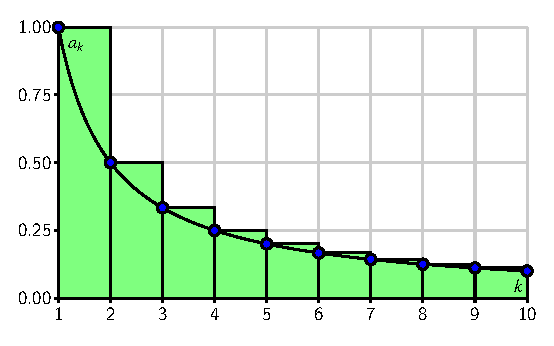
\includegraphics{figures/8_3_Integral_test1.eps}}
%\hspace{0.2in} \resizebox{!}{1.25in}{\includegraphics{figures/8.3_Integral_test2.eps}}
\caption{A picture of the 9th partial sum of the harmonic series as a sum of areas of rectangles.}
\label{F:8.3.4_Integral_Test}
\end{center}
\end{figure}
The graph of the continuous function $f$ defined by $f(x) = \frac{1}{x}$ is overlaid on this plot. 
\ba
\item Explain how this picture represents a particular Riemann sum.
\item What is the definite integral that corresponds to the Riemann sum you considered in (a)?
\item Which is larger, the definite integral in (b), or the corresponding partial sum $S_9$ of the series? Why?

\item If instead of considering the 9th partial sum, we consider the $n$th partial sum, and we let $n$ go to infinity, we can then compare the series $ \sum_{k=1}^{\infty} \frac{1}{k}$ to the improper integral $ \int_{1}^{\infty} \frac{1}{x} \ dx$.  Which of these quantities is larger?  Why?

\item Does the improper integral $ \int_{1}^{\infty} \frac{1}{x} \ dx$ converge or diverge? What does that result, together with your work in (d), tell us about the series $ \sum_{k=1}^{\infty} \frac{1}{k}$?

\ea
\end{activity}

\begin{smallhint}
\ba
	\item Small hints for each of the prompts above.
\ea
\end{smallhint}
\begin{bighint}
\ba
	\item Big hints for each of the prompts above.
\ea
\end{bighint}
\begin{activitySolution}
\ba
	\item Notice that the $n$th partial sum of the series $\ds \sum_{k=1}^{\infty} \frac{1}{k}$ is equal to the left hand Riemann sum of $f(x)$ on the interval $[1,n]$.
    \item Since $f$ is a decreasing function, it follows that
\[\ds \sum_{k=1}^{n} \frac{1}{k} > \int_{1}^{n} \frac{1}{x} \ dx.\]
    \item Letting Since $f$ is decreasing, the improper integral $\ds \int_{1}^{\infty} \frac{1}{x} \ dx$ is smaller than the limit of the Riemann sums as $n$ goes to infinity. So  we wind up with a comparison between the series $\ds \sum_{k=1}^{\infty} \frac{1}{n}$ and the improper integral:
\[\ds \sum_{k=1}^{\infty} \frac{1}{k} > \int_{1}^{\infty} \frac{1}{x} \ dx.\]
    \item We can evaluate the improper integral as follows:
\begin{align*}
\int_{1}^{\infty} f(x) \ dx &= \lim_{t \to \infty} \int_{1}^{t} \frac{1}{x} \ dx \\
    &= \lim_{t \to \infty} \ln(x) |_{1}^{t} \\
    &= \lim_{t \to \infty} \left(\ln(t) - \ln(1) \right) \\
    &= \infty.
\end{align*}
Since the value of the series $\ds \sum_{k=1}^{\infty} \frac{1}{k}$ exceeds the value of the infinite improper integral, we must conclude that the series $\ds \sum_{k=1}^{\infty} \frac{1}{k}$ diverges.
\ea
\end{activitySolution}
\aftera 

The ideas from Activity \ref{8.3.Act4} hold more generally.  Suppose that $f$  is a continuous decreasing function and that $a_k = f(k)$ for each value of $k$.  Consider the corresponding series $ \sum_{k=1}^{\infty} a_k$. The partial sum
\[S_n = \sum_{k=1}^{n} a_k\]
can always be viewed as a left hand Riemann sum of $f(x)$ using rectangles with heights given by the values $a_k$ and bases of length 1. A representative picture is shown at left in Figure \ref{F:8.3.Integral_Test}. Since $f$ is a decreasing function, we have that
\[S_n > \int_1^n f(x) \ dx.\]
Taking limits as $n$ goes to infinity shows that
\[\sum_{k=1}^{\infty} a_k > \int_{1}^{\infty} f(x) \ dx.\]
Therefore, if the improper integral $ \int_{1}^{\infty} f(x) \ dx$ diverges, so does the series $ \sum_{k=1}^{\infty} a_k$.
\begin{figure}[h]
\begin{center}
\resizebox{!}{1.5in}{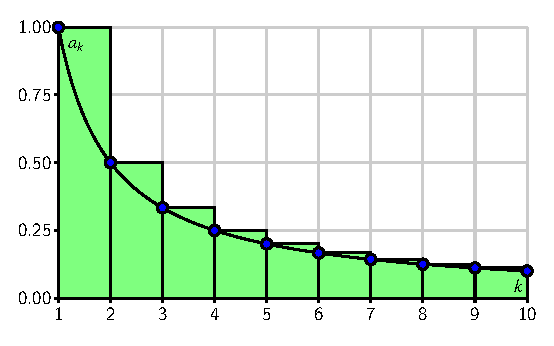
\includegraphics{figures/8_3_Integral_test1.eps}} \hspace{0.25in} \resizebox{!}{1.5in}{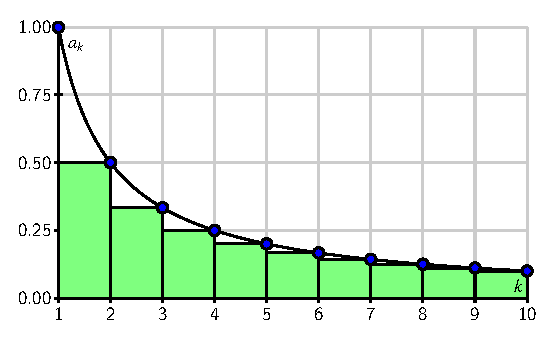
\includegraphics{figures/8_3_Integral_test2.eps}}
\caption{Comparing an improper integral to a series}
\label{F:8.3.Integral_Test}
\end{center}
\end{figure}

What's more, if we look at the right hand Riemann sums of $f$ on $[1,n]$ as shown at right in Figure \ref{F:8.3.Integral_Test}, we see that
\[\int_{1}^{\infty} f(x) \ dx >  \sum_{k=2}^{\infty} a_k.\]
So if $ \int_{1}^{\infty} f(x) \ dx$ converges, then so does $ \sum_{k=2}^{\infty} a_k$, which also means that the series $ \sum_{k=1}^{\infty} a_k$ converges. Our preceding discussion has demonstrated the truth of the Integral Test\index{integral test}.

\vspace*{5pt}
\nin \framebox{\hspace*{3 pt}
\parbox{\boxwidth}{
\textbf{The Integral Test. } Let $f$ be a real valued function and assume $f$ is decreasing and positive for all $x$ larger than some number $c$.  Let $a_k = f(k)$ for each positive integer $k$. 
\begin{enumerate}
\item If the improper integral $ \int_{c}^{\infty} f(x) \, dx$ converges, then the series $ \sum_{k=1}^{\infty} a_k$ converges.
\item If the improper integral $ \int_{c}^{\infty} f(x) \, dx$ diverges, then the series $ \sum_{k=1}^{\infty} a_k$ diverges.
\end{enumerate}
} \hspace*{3 pt}}
\vspace*{1pt}

Note that the Integral Test compares a given infinite series to a natural, corresponding improper integral and basically says that the infinite series and corresponding improper integral both have the same convergence status.  In the next activity, we apply the Integral Test to determine the convergence or divergence of a class of important series.

\newpage

\begin{activity} \label{8.3.Act5} The series $\sum \frac{1}{k^p}$ are special series called $p$-series. We have already seen that the $p$-series with $p=1$ (the harmonic series) diverges. We investigate the behavior of other $p$-series in this activity.
\ba
    \item Evaluate the improper integral $ \int_1^{\infty} \frac{1}{x^2} \ dx$. Does the series $ \sum_{k=1}^{\infty} \frac{1}{k^2}$
converge or diverge? Explain.


    \item Evaluate the improper integral $ \int_1^{\infty} \frac{1}{x^p} \ dx$ where $p > 1$. For which values of $p$ can we conclude that the series $ \sum_{k=1}^{\infty} \frac{1}{k^p}$
converges? 

    \item Evaluate the improper integral $ \int_1^{\infty} \frac{1}{x^p} \ dx$ where $p < 1$. What does this tell us about the corresponding $p$-series
$ \sum_{k=1}^{\infty} \frac{1}{k^p}$?

\item Summarize your work in this activity by completing the following statement.
\begin{quote}
The $p$-series $ \sum_{k=1}^{\infty} \frac{1}{k^p}$ converges if and only if \underline{\hspace{2in}}.
\end{quote}

\ea
\end{activity}

\begin{smallhint}
\ba
	\item Small hints for each of the prompts above.
\ea
\end{smallhint}
\begin{bighint}
\ba
	\item Big hints for each of the prompts above.
\ea
\end{bighint}
\begin{activitySolution}
\ba
	\item We evaluate the improper integral:
\begin{align*}
\int_{1}^{\infty} \frac{1}{x^2} \ dx &= \lim_{t \to \infty} \int_{1}^{t} \frac{1}{x^2} \ dx \\
    &= \lim_{t \to \infty} -\frac{1}{x} \biggm|_{1}^{t} \\
    &= \lim_{t \to \infty} \left(-\frac{1}{t} + \frac{1}{1} \right) \\
    &= 1.
\end{align*}
So the improper integral converges. The Integral Test then shows that the series $ \sum_{k=1}^{\infty} \frac{1}{k^2}$ converges.
    \item Assume $p > 1$. Then $p-1 > 0$ and so $x^{-p+1} = \frac{1}{x^{p-1}}$ and
\[ \lim_{x \to \infty} x^{-p+1} = \lim_{x \to \infty} \frac{1}{x^{p-1}} = 0.\]
Thus,
\begin{align*}
\int_{1}^{\infty} \frac{1}{x^p} \ dx &= \lim_{t \to \infty} \int_{1}^{t} \frac{1}{x^p} \ dx \\
    &= \lim_{t \to \infty} \frac{x^{-p+1}}{-p+1} \biggm|_{1}^{t} \\
    &= \frac{1}{1-p} \lim_{t \to \infty} \left(t^{-p+1} -  1 \right) \\
    &= \frac{1}{p-1}.
\end{align*}
So the improper integral $ \int_1^{\infty} \frac{1}{x^p} \ dx$ converges when $p > 1$. The Integral Test then shows that the series $ \sum_{k=1}^{\infty} \frac{1}{k^p}$ converges when $p > 1$.
    \item Assume $p < 1$. Then $1-p > 0$ and so
\[ \lim_{x \to \infty} x^{-p+1} = \infty.\]
Thus,
\begin{align*}
\int_{1}^{\infty} \frac{1}{x^p} \ dx &= \lim_{t \to \infty} \int_{1}^{t} \frac{1}{x^p} \ dx \\
    &= \lim_{t \to \infty} \frac{x^{-p+1}}{-p+1} \biggm|_{1}^{t} \\
    &= \frac{1}{1-p} \lim_{t \to \infty} \left(t^{-p+1} -  1 \right) \\
    &= \infty.
\end{align*}
So the improper integral $ \int_1^{\infty} \frac{1}{x^p} \ dx$ diverges when $p < 1$. The Integral Test then shows that the series $ \sum_{k=1}^{\infty} \frac{1}{k^p}$ also diverges when $p < 1$.
    \item We complete the statement as
\begin{quote}
The $p$-series $ \sum_{k=1}^{\infty} \frac{1}{k^p}$ converges if and only if $p > 1$.
\end{quote}
\ea
\end{activitySolution}
\aftera 

\subsection*{The Limit Comparison Test}\index{limit comparison test}

The Integral Test allows us to determine the convergence of an entire family of series: the $p$-series. However, we have seen that it is, in general, difficult to integrate functions, so the Integral Test is not one that we can use all of the time. In fact, even for a relatively simple series like $ \sum \frac{k^2+1}{k^4+2k+2}$, the Integral Test is not an option. In this section we will develop a test that we can use to apply to series of rational functions like this by comparing their behavior to the behavior of $p$-series.

\begin{activity} \label{8.3.Act6} Consider the series $ \sum \frac{k+1}{k^3+2}$. Since the convergence or divergence of a series only depends on the behavior of the series for large values of $k$, we might examine the terms of this series more closely as $k$ gets large.
    \ba
    \item By computing the value of $ \frac{k+1}{k^3+2}$ for $k = 100$ and $k = 1000$, explain why the terms $ \frac{k+1}{k^3+2}$ are essentially $ \frac{k}{k^3}$ when $k$ is large. 

    \item Let's formalize our observations in (a) a bit more. Let $a_k =  \frac{k+1}{k^3+2}$ and $b_k =  \frac{k}{k^3}$. Calculate 
    \[\lim_{k \to \infty} \frac{a_k}{b_k}.\]
    What does the value of the limit tell you about $a_k$ and $b_k$ for large values of $k$? Compare your response from part (a). 

    \item Does the series $ \sum \frac{k}{k^3}$ converge or diverge? Why? What do you think that tells us about the convergence or divergence of the series $ \sum \frac{k+1}{k^3+2}$? Explain. 

\ea
\end{activity}

\begin{smallhint}
\ba
	\item Small hints for each of the prompts above.
\ea
\end{smallhint}
\begin{bighint}
\ba
	\item Big hints for each of the prompts above.
\ea
\end{bighint}
\begin{activitySolution}
\ba
	\item When $k$ is very large, the constant 1 in the numerator is negligible compared to $k$ and the constant 2 in the denominator is negligible compared to $k^3$. So the numerator looks like $k$ and the denominator $k^3$ when $k$ is large. It follows that $ \frac{k+1}{k^3+2}$ looks like $ \frac{k}{k^3}$ when $k$ is large.
    \item Note that 
    \begin{align*}
    \lim_{k \to \infty} \frac{a_k}{b_k} &= \lim_{k \to \infty} \frac{ \frac{k+1}{k^3+2} }{ \frac{k}{k^3} } \\
        &= \lim_{k \to \infty} \frac{(k+1)k^3}{k(k^3+2)} \\
        &= \lim_{k \to \infty} \frac{1+\frac{1}{k}}{1+\frac{2}{k}} \\
        &= 1.
    \end{align*}
    This tells us that $a_k \approx b_k$ for large values of $k$, which is what we suggested in part (a). 
    \item Since $\frac{k}{k^3} = \frac{1}{k^2}$, the series $ \sum \frac{k}{k^3}$ is a $p$-series with $p=2$ and so converges. Since $a_k \approx b_k$ for large values of $k$, it seems reasonable to expect that $\sum a_k \approx \sum b_k$ for large $k$s. Since $\sum a_k$ is finite, we should then conclude that $\sum b_k$ is also finite. So $ \sum \frac{k+1}{k^3+2}$ should be a convergent series. 
\ea
\end{activitySolution}
\aftera 

Activity \ref{8.3.Act6} illustrates how we can compare one series with positive terms to another whose behavior (that is, whether the series converges or diverges) we know. More generally, suppose we have two series $\sum a_k$ and $\sum b_k$ with positive terms and we know the behavior of the series $\sum a_k$. Recall that the convergence or divergence of a series depends only on what happens to the terms of the series for large values of $k$, so if we know that $a_k$ and $b_k$ are essentially proportional to each other for large $k$, then the two series $\sum a_k$ and $\sum b_k$
should behave the same way. In other words, if there is a positive finite constant $c$ such that
\[\lim_{k \to \infty} \frac{b_k}{a_k} = c,\]
then $b_k \approx ca_k$ for large values of $k$. So
\[\sum b_k \approx \sum ca_k = c  \sum a_k.\]
Since multiplying by a nonzero constant does not affect the convergence or divergence of a series, it follows that the series $\sum a_k$ and $\sum b_k$ either both converge or both diverge. The formal statement of this fact is called the Limit Comparison Test.


\vspace*{5pt}
\nin \framebox{\hspace*{3 pt}
\parbox{\boxwidth}{
\textbf{The Limit Comparison Test.} Let $\sum a_k$ and $\sum b_k$ be series with positive terms. If
\[\lim_{k \to \infty} \frac{b_k}{a_k} = c\]
for some positive (finite) constant $c$, then $ \sum a_k$ and $ \sum b_k$
either both converge or both diverge.
} \hspace*{3 pt}}
\vspace*{1pt}

In essence, the Limit Comparison Test shows that if we have a series $\sum \frac{p(k)}{q(k)}$ of rational functions where $p(k)$ is a polynomial of degree $m$ and $q(k)$ a polynomial of degree $l$, then the series $\sum \frac{p(k)}{q(k)}$ will behave like the series $\sum \frac{k^m}{k^l}$. So this test allows us to quickly and easily determine the convergence or divergence of series whose summands are rational functions.

\begin{activity} \label{8.3.Act7} Use the Limit Comparison Test to determine the convergence or divergence of the series
\[\sum \frac{3k^2+1}{5k^4+2k+2}.\]
by comparing it to the series $ \sum \frac{1}{k^2}$.

\end{activity}

\begin{smallhint}
\ba
	\item Small hints for each of the prompts above.
\ea
\end{smallhint}
\begin{bighint}
\ba
	\item Big hints for each of the prompts above.
\ea
\end{bighint}
\begin{activitySolution}
Let $b_k = \frac{k^2+1}{k^4+2k+2}$ and $a_k = \frac{1}{k^2}$. Then
\begin{align*}
\lim_{k \to \infty} \frac{b_k}{a_k} &= \lim_{k \to \infty} \frac{\frac{k^2+1}{k^4+2k+2}}{\frac{1}{k^2}} \\
    &= \lim_{k \to \infty} \frac{k^4+k^2}{k^4+2k+2} \\
    &= \lim_{k \to \infty} \frac{1+\frac{1}{k^2}}{1+\frac{2}{k^3}+\frac{2}{k^4}} \\
    &= 1.
\end{align*}
 Since $ \lim_{k \to \infty} \frac{b_k}{a_k}$ is a finite positive constant, the Limit Comparison Test shows that $ \sum \frac{1}{k^2}$ and $ \sum \frac{k^2+1}{k^4+2k+2}$ either both converge or both diverge. We know that $ \sum \frac{1}{k^2}$ is a $p$-series with $p > 1$ and so $ \sum \frac{1}{k^2}$  converges. Therefore, the series $ \sum \frac{k^2+1}{k^4+2k+2}$ also converges.
\end{activitySolution}
\aftera 


\subsection*{The Ratio Test} \index{ratio test}
The Limit Comparison Test works well if we can find a series with known behavior to compare. But such series are not always easy to find. In this section we will examine a test that allows us to examine the behavior of a series by comparing it to a geometric series, without knowing in advance which geometric series we need.

\begin{activity} \label{8.3.Act8} Consider the series defined by
\begin{equation} \label{eq:8.3_ratio_example}
\sum_{k=1}^{\infty} \frac{2^k}{3^k-k}.
\end{equation}
This series is not a geometric series, but this activity will illustrate how we might compare this series to a geometric one. Recall that a series $\sum a_k$ is geometric if the ratio $\frac{a_{k+1}}{a_k}$ is always the same. For the series in (\ref{eq:8.3_ratio_example}), note that $a_k = \frac{2^k}{3^k-k}$.
\ba
\item  To see if $\sum \frac{2^k}{3^k-k}$ is comparable to a geometric series, we analyze the ratios of successive terms in the series. Complete Table \ref{T:8.3.3_ratio_test}, listing your calculations to at least 8 decimal places.
\begin{table}[ht]
\begin{center}
\renewcommand{\arraystretch}{1.5}
\begin{tabular}{c|p{2in}}
$k$   & $\frac{a_{k+1}}{a_k}$ \\
5   & \\
10   &  \\
20   &  \\
21   &  \\
22   &  \\
23  & \\
24   &  \\
25   &  \\
\end{tabular}
\caption{Ratios of successive terms in the series $\sum \frac{2^k}{3^k-k}$}
\label{T:8.3.3_ratio_test}
\end{center}
\end{table}

\item Based on your calculations in Table \ref{T:8.3.3_ratio_test}, what can we say about the ratio $\frac{a_{k+1}}{a_k}$ if $k$ is large?

\item Do you agree or disagree with the statement: ``the series $\sum \frac{2^k}{3^k-k}$ is approximately geometric when $k$ is large''? If not, why not? If so, do you think the series $\sum \frac{2^k}{3^k-k}$ converges or diverges? Explain.



\ea
\end{activity}

\begin{smallhint}
\ba
	\item Small hints for each of the prompts above.
\ea
\end{smallhint}
\begin{bighint}
\ba
	\item Big hints for each of the prompts above.
\ea
\end{bighint}
\begin{activitySolution}
\ba
	\item Ratios of successive summands in the series are shown (to 10 decimal places) in the following table. 
%\begin{table}[ht]
\begin{center}
\renewcommand{\arraystretch}{1.5}
\begin{tabular}{c|p{2in}}
$k$   & $\frac{a_{k+1}}{a_k}$ \\
5   & 0.6583679115 \\
10   & 0.6665951585 \\
20   & 0.6666666642 \\
21   & 0.6666666658 \\
22   & 0.6666666664  \\
23  & 0.6666666666 \\
24   & 0.6666666666 \\
25   & .6666666667 \\
\end{tabular}
%\label{T:8.3.3_ratio_test_b}
%\caption{Ratios of successive summands in the series $\sum \frac{2^k}{3^k-k}$}
\end{center}
%\end{table}
    \item The calculations in the table in part (a) seem to indicate that the ratio $\frac{a_{k+1}}{a_k}$ is roughly $\frac{2}{3}$ when $k$ is large.
    \item Since $\frac{a_{k+1}}{a_k} \approx \frac{2}{3}$ for large $k$, the series $\sum \frac{2^k}{3^k-k}$ is approximately the same as $\sum \left(\frac{2}{3}\right)^k$ when $k$ is large. So the series $\sum \frac{2^k}{3^k-k}$ is approximately geometric with ratio $\frac{2}{3}$ when $k$ is large. Since the series $\sum \left(\frac{2}{3}\right)^k$ converges because the ratio is less than 1, we expect that the series $\sum \frac{2^k}{3^k-k}$ will also converge.
\ea
\end{activitySolution}
\aftera 

We can generalize the argument in Activity \ref{8.3.Act8} in the following way. Consider the series $ \sum a_k.$
If
\[\frac{a_{k+1}}{a_k} \approx r\]
for large values of $k$, then $a_{k+1} \approx ra_k$ for large $k$ and the series $\sum a_k$ is approximately the geometric series $\sum ar^k$ for large $k$. Since the geometric series with ratio $r$ converges only for $-1 <  r < 1$, we see that the series $ \sum a_k$
will converge if
\[\lim_{k \to \infty} \frac{a_{k+1}}{a_k} = r\]
for a value of $r$ such that $|r| < 1$. This result is known as the Ratio Test.

\vspace*{5pt}
\nin \framebox{\hspace*{3 pt}
\parbox{\boxwidth}{
\textbf{The Ratio Test. } Let $ \sum a_k$
 be an infinite series. Suppose
\[\lim_{k \to \infty} \frac{|a_{k+1}|}{|a_k|} = r.\]
\begin{enumerate}
\item If $0 \leq r < 1$, then the series $\sum a_k$ converges.
\item If $1 < r$, then the series $\sum a_k$ diverges.
\item If $r = 1$, then the test is inconclusive.
\end{enumerate}
} \hspace*{3 pt}}
\vspace*{1pt}

{\bf Note well:}  The Ratio Test takes a given series and looks at the limit of the ratio of consecutive terms; in so doing, the test is essentially asking, ``is this series approximately geometric?''  If the series can be thought of as essentially geometric, the test use the limiting common ratio to determine if the given series converges.

We have now encountered several tests for determining convergence or divergence of series. The Divergence Test can be used to show that a series diverges, but never to prove that a series converges. We used the Integral Test to determine the convergence status of an entire class of series, the $p$-series. The Limit Comparison Test works well for series that involve rational functions and which can therefore by compared to $p$-series.  Finally, the Ratio Test allows us to compare our series to a geometric series; it is particularly useful for series that involve $n$th powers and factorials.  Two other tests, the Direct Comparison Test and the Root Test, are discussed in the exercises. Now it is time for some practice.

\begin{activity} \label{8.3.Act9} Determine whether each of the following series  converges or diverges. Explicitly state which test you use.
\ba
\item $\ds \sum \frac{k}{2^k}$

\item $\ds \sum \frac{k^3+2}{k^2+1}$

\item $\ds \sum \frac{10^k}{k!}$

\item $\ds \sum \frac{k^3-2k^2+1}{k^6+4}$

\ea
\end{activity}

\begin{smallhint}
\ba
	\item Small hints for each of the prompts above.
\ea
\end{smallhint}
\begin{bighint}
\ba
	\item Big hints for each of the prompts above.
\ea
\end{bighint}
\begin{activitySolution}
\ba
	\item Since $\lim_{n \to \infty} \frac{n}{2^n} = 0$, the Divergence Test does not apply. The Ratio Test is a good one to apply with series whose terms involve exponentials and polynomials.

In this example we have $a_{n+1} = \frac{n+1}{2^{n+1}}$ and $a_n = \frac{n}{2^n}$. So
\[\frac{a_{n+1}}{a_n} = \frac{\frac{n+1}{2^{n+1}}}{\frac{n}{2^n}} = \frac{n+1}{2n}.\]
As $n$ goes to infinity, the fraction $\frac{n+1}{n}$ goes to 1 and so
\[\lim_{n \to \infty} \frac{n+1}{2n} = \frac{1}{2}.\]
So in this example, for large $n$ we have that $\frac{a_{n+1}}{a_n} \approx \frac{1}{2}$ or that $\sum a_n$ is roughly a geometric series for large $n$ with ratio $\frac{1}{2}$. Since geometric series with ratio $\frac{1}{2}$ converges, we can conclude that
\[\sum \frac{n}{2^n}\]
converges as well.

\item For this series, notice that the degree of the numerator is greater than the degree of the denominator, so
\[\lim_{n \to \infty} \frac{n^3+2}{n^2+1} = \infty.\]
Since this limit is not 0, the Divergence Test shows that $\ds \sum \frac{k^3+2}{k^2+1}$ diverges.

\item We use the Ratio Test here with $a_k = \frac{10^k}{k!}$. Now
\begin{align*}
\lim_{k \to \infty} \frac{a_{k+1}}{a_k} &= \lim_{k \to \infty} \frac{ \frac{10^{k+1}}{(k+1)!} }{ \frac{10^k}{k!} } \\
    &= \lim_{k \to \infty} \frac{10^{k+1}(k!)}{10^k(k+1)!} \\
    &= \lim_{k \to \infty} \frac{10}{k+1} \\
    &= 0,
\end{align*}
so the Ratio Test shows that $\ds \sum \frac{10^k}{k!}$ converges.

\item If we ignore the highest powered terms, then the series $\ds \sum \frac{k^3-2k^2+1}{k^6+4}$ looks like the series $\ds \sum \frac{k^3}{k^6} = \sum \frac{1}{k^3}$. We formally apply the Limit Comparison Test as follows:
\begin{align*}
\lim_{k \to \infty} \frac{ \frac{k^3-2k^2+1}{k^6+4} }{  \frac{1}{k^3} } &= \lim_{k \to \infty} \frac{k^6-2k^5+k^3}{k^6+4} \\
    &= \lim_{k \to \infty} \frac{1 - \frac{2}{k} + \frac{1}{k^3}}{1 + \frac{4}{k^6}} \\
    & 1.
\end{align*}
Since $\ds \sum \frac{1}{k^3}$ is a $p$-series with $p=3>1$, the series $\ds \sum \frac{1}{k^3}$ converges. Consequently, the Limit Comparison Test shows that $\ds \sum \frac{k^3-2k^2+1}{k^6+4}$ converges as well. 

\ea
\end{activitySolution}
\aftera 

%If you choose to include a worked example, please use this style:

%\bex \label{Ex:8.1.1}
%Suppose that $\ldots$
%\eex
%Here is the provided solution to the example.
%\afterex






%\nin \framebox{\hspace*{3 pt}
%\parbox{6.25 in}{
\begin{summary}
\item An infinite series is a sum of the elements in an infinite sequence. In other words, an infinite series is a sum of the form
\[a_1 + a_2 + \cdots + a_n + \cdots = \sum_{k=1}^{\infty} a_k\]
where $a_k$ is a real number for each positive integer $k$.
\item The $n$th partial sum $S_n$ of the series $\sum_{k=1}^{\infty} a_k$ is the sum of the first $n$ terms of the series. That is,
\[S_n = a_1+a_2+ \cdots + a_n = \sum_{k=1}^{\infty} a_k.\]
\item The sequence $\{S_n\}$ of partial sums of a series $\sum_{k=1}^{\infty} a_k$ tells us about the convergence or divergence of the series.  In particular
	\begin{itemize}
	\item[-] The series $\sum_{k=1}^{\infty} a_k$ converges if the sequence $\{S_n\}$ of partial sums converges. In this case we say that the series is the limit of the sequence of partial sums and write
	\[\sum_{k=1}^{\infty} a_k =\lim_{n \to \infty} S_n.\]
	\item[-] The series $\sum_{k=1}^{\infty} a_k$ diverges if the sequence $\{S_n\}$ of partial sums diverges.
	\end{itemize}
\end{summary}
%} \hspace*{3 pt}}

\nin \hrulefill

\begin{exercises}

\item In this exercise we investigate the sequence $\left\{\frac{b^n}{n!}\right\}$ for any constant $b$.
    \ba
    \item Use the Ratio Test to determine if the series $\sum \frac{10^k}{k!}$ converges or diverges.

\begin{exerciseSolution}

\solution We use the Ratio Test with $a_n = \frac{10^n}{n!}$. First we consider the ratios of successive terms:
\begin{eqnarray*}
\lim_{n \to \infty} \frac{a_{n+1}}{a_n} &=& \lim_{n \to \infty} \frac{ \frac{10^{n+1}}{(n+1)!}}{ \frac{10^{n}}{(n)!} } \\
    &=& \lim_{n \to \infty} \frac{10}{n+1} \\
    &=& 0.
\end{eqnarray*}
Since the limit of the ratio of successive terms is less than 1, we conclude that the series $\sum \frac{10^k}{k!}$ converges.

\end{exerciseSolution}

\item Now apply the Ratio Test to determine if the series $\sum \frac{b^k}{k!}$ converges for any constant $b$.

\begin{exerciseSolution}

\solution We use the Ratio Test with $a_n = \frac{b^n}{n!}$. First we consider the ratios of successive terms:
\begin{align*}
\lim_{n \to \infty} \frac{a_{n+1}}{a_n} &= \lim_{n \to \infty} \frac{ \frac{b^{n+1}}{(n+1)!} }{ \frac{b^{n}}{(n)!} } \\
    &= \lim_{n \to \infty} \frac{b}{n+1} \\
    &= 0.
\end{align*}
Since the limit of the ratio of successive terms is less than 1, we conclude that the series $\sum \frac{b^k}{k!}$ converges.

\end{exerciseSolution}

\item Use your result from (b) to decide whether the sequence  $\left\{\frac{b^n}{n!}\right\}$ converges or diverges. If the sequence $\left\{\frac{b^n}{n!}\right\}$ converges, to what does it converge? Explain your reasoning.

\begin{exerciseSolution}

\solution Since the series $\sum \frac{b^n}{n!}$ converges, the Divergence Test tells us that the sequence $\left\{\frac{b^n}{n!}\right\}$ has to converge to 0.

\end{exerciseSolution}

\ea

  \item \label{ex:8.3_Root_Test} There is a test for convergence similar to the Ratio Test called the \emph{Root Test}. Suppose we have a series $ \sum a_k$ of positive terms so that $a_n \to 0$ as $n \to \infty$.
  \ba
  \item Assume
  \[\sqrt[n]{a_n} \to r\]
as $n$ goes to infinity. Explain why this tells us that $a_n \approx r^n$ for large values of $n$.

\begin{exerciseSolution}

If $\sqrt[n]{a_n} \to r$, then as $n$ increases we know that $\sqrt[n]{a_n} \approx r$. So for large $n$ we have $a_n \approx r^n$.

\end{exerciseSolution}

\item Using the result of part (a), explain why $\sum a_k$ looks like a geometric series when $n$ is big. What is the ratio of the geometric series to which $\sum a_k$ is comparable?

\begin{exerciseSolution}

Since $a_n \approx r^n$ when $n$ is large,
\[\sum a_k \approx \sum r^k\]
when $k$ is large. So $\sum a_k$ looks like a geometric sequence with ratio $r$ when $n$ is big.

\end{exerciseSolution}

\item Use what we know about geometric series to determine that values of $r$ so that $\sum a_k$ converges if $\sqrt[n]{a_n} \to r$ as $n \to \infty$.

\begin{exerciseSolution}

Since the terms in our series are all positive, we must have $r > 0$.  Now the geometric series with ratio $r$ converges only for $r < 1$,so the series
\[\sum a_k\]
will converge if
\[\lim_{n \to \infty} \sqrt[n]{a_n} = r\]
with $0 < r < 1$.

\end{exerciseSolution}

\ea	

\item The associative and distributive laws of addition allow us to add finite sums in any order we want. That is, if $ \sum_{k=0}^n a_k$ and $ \sum_{k=0}^n b_k$ are finite sums of real numbers, then
\[\sum_{k=0}^{n} a_k + \sum_{k=0}^n b_k = \sum_{k=0}^n (a_k+b_k).\]
However, we do need to be careful extending rules like this to infinite series.
\ba
\item Let $a_n =  1 + \frac{1}{2^n}$ and $b_n = -1$ for each nonnegative integer $n$.
    \begin{itemize}
    \item[(i)] Explain why the series $ \sum_{k=0}^{\infty} a_k$ and $ \sum_{k=0}^{\infty} b_k$ both diverge. 
    
    \item[(ii)] Explain why the series $ \sum_{k=0}^{\infty} (a_k+b_k)$ converges.

    \item[(iii)] Explain why
\[\sum_{k=0}^{\infty} a_k + \sum_{k=0}^{\infty} b_k \neq \sum_{k=0}^{\infty} (a_k+b_k).\]
This shows that it is possible to have to two divergent series $ \sum_{k=0}^{\infty} a_k$ and $ \sum_{k=0}^{\infty} b_k$ but yet have the series $ \sum_{k=0}^{\infty} (a_k+b_k)$ converge.
    \end{itemize}

\item While part (a) shows that we cannot add series term by term in general, we can under reasonable conditions. The problem in part (a) is that we tried to add divergent series. In this exercise we will show that if $\sum a_k$ and $\sum b_k$ are convergent series, then $\sum (a_k+b_k)$ is a convergent series and
\[\sum (a_k+b_k) = \sum a_k + \sum b_k.\]
    \begin{itemize}
    \item[(i)] Let $A_n$ and $B_n$ be the $n$th partial sums of the series $\sum_{k=1}^{\infty} a_k$ and $\sum_{k=1}^{\infty} b_k$, respectively. Explain why
\[A_n + B_n = \sum_{k=1}^n (a_k+b_k).\]

    \item[(ii)] Use the previous result and properties of limits to show that
\[\sum_{k=1}^{\infty} (a_k+b_k) = \sum_{k=1}^{\infty} a_k + \sum_{k=1}^{\infty} b_k.\]
(Note that the starting point of the sum is irrelevant in this problem, so it doesn't matter where we begin the sum.)

        \end{itemize}

\item Use the prior result to find the sum of the series $ \sum_{k=0}^{\infty} \frac{2^k+3^k}{5^k}$.

\ea

\item \label{ex:8.3_Direct_Comparison_Test} Series are sums, just like improper integrals. Recall that we had a comparison test for improper integrals, so it is reasonable to expect that we could have a similar test for infinite series. We consider such a test in this exercise. First we consider an example.
    \ba
    \item Consider the series
\[\sum \frac{1}{k^2} \hspace{0.5in} \text{ and } \hspace{0.5in} \sum \frac{1}{k^2+k}.\]
We know that the series $ \sum \frac{1}{k^2}$ is a $p$-series with $p = 2 > 1$ and so $ \sum \frac{1}{k^2}$ converges. In this part of the exercise we will see how to use information about $ \sum \frac{1}{k^2}$ to determine information about $ \sum \frac{1}{k^2+k}$. Let $a_k = \frac{1}{k^2}$ and $b_k = \frac{1}{k^2+k}$.
        \begin{itemize}
        \item[(i)] Let $S_n$ be the $n$th partial sum of $ \sum \frac{1}{k^2}$ and $T_n$ the $n$th partial sum of $ \sum \frac{1}{k^2+k}$. Which is larger, $S_1$ or $T_1$? Why?

\begin{exerciseSolution}
Since $S_1 = 1$ and $T_1 = \frac{1}{2}$, we see that $S_1 > T_1$.
\end{exerciseSolution}

        \item[(ii)] Recall that
\[S_2 = S_1 + a_2 \hspace{0.5in} \text{ and } \hspace{0.5in} T_2 = T_1 + b_2.\]
Which is larger, $a_2$ or $b_2$? Based on that answer, which is larger, $S_2$ or $T_2$?

\begin{exerciseSolution}
Since $a_2 = \frac{1}{4}$ and $b_2 = \frac{1}{6}$, it is the case that $a_2 > b_2$. We already know that $S_1 > T_1$, so adding a larger number to $S_1$ than we add to $T_1$ makes $S_2 > T_2$.
\end{exerciseSolution}

        \item[(iii)] Recall that
\[S_3 = S_2 + a_3 \hspace{0.5in} \text{ and } \hspace{0.5in} T_3 = T_2 + b_3.\]
Which is larger, $a_3$ or $b_3$? Based on that answer, which is larger, $S_3$ or $T_3$?

\begin{exerciseSolution}
Since $a_3 = \frac{1}{9}$ and $b_3 = \frac{1}{12}$, it is the case that $a_3 > b_3$. We already know that $S_2 > T_2$, so adding a larger number to $S_2$ than we add to $T_2$ makes $S_3 > T_3$.
\end{exerciseSolution}

        \item[(iv)] Which is larger, $a_n$ or $b_n$? Explain. Based on that answer, which is larger, $S_n$ or $T_n$?

\begin{exerciseSolution}
Since $n^2+n > n^2$ when $n$ is positive, we have $\frac{1}{n^2} > \frac{1}{n^2+n}$ or $a_n > b_n$. So at each step, we are adding larger numbers to the partial sums of $ \sum \frac{1}{k^2}$ than we are to the partial sums of $ \sum \frac{1}{k^2+k}$, we conclude that $S_n > T_n$.
\end{exerciseSolution}

        \item[(v)] Based on your response to the previous part of this exercise, what relationship do you expect there to be between $ \sum \frac{1}{k^2}$ and  $ \sum \frac{1}{k^2+k}$? Do you expect $ \sum \frac{1}{k^2+k}$ to converge or diverge? Why?

\begin{exerciseSolution}
Since $S_n > T_n$, we should expect $ \lim_{n \to \infty} S_n > \lim_{n \to \infty} T_n$ or
\[ \sum \frac{1}{k^2} >  \sum \frac{1}{k^2+k}.\]
Since $ \sum \frac{1}{k^2}$ is a $p$-series with $p=2 > 1$, we know that $ \sum \frac{1}{k^2}$ converges (and is finite). Now $ \sum \frac{1}{k^2+k}$ is a sum of positive terms and is therefore positive, and is also less than a finite number ($ \sum \frac{1}{k^2}$), so we expect that $ \sum \frac{1}{k^2+k}$ converges as well.
\end{exerciseSolution}

        \end{itemize}

    \item The example in the previous part of this exercise illustrates a more general result. Explain why the Direct Comparison Test, stated here, works.
    
\vspace*{5pt}
\nin \framebox{\hspace*{3 pt}
\parbox{4.6in}{
\textbf{The Direct Comparison Test. } If
\[0 \leq b_k \leq a_k\]
for every $k$, then we must have
\[0 \leq \sum b_k \leq \sum a_k\]
\begin{enumerate}
\item If $\sum a_k$ converges, then $\sum b_k$ converges.
\item If $\sum b_k$ diverges, then $\sum a_k$ diverges.
\end{enumerate}
} \hspace*{3 pt}}
\vspace*{1pt}

\noindent \textbf{Important Note:} This comparison test applies only to series with nonnegative terms.

\begin{exerciseSolution}
If we have two series $\sum a_k$ and $\sum b_k$ of positive terms with $a_k \geq b_k$ for every $k$, then
\[\sum a_k \geq \sum b_k > 0.\]
Now if $\sum b_k$ diverges, then $\sum b_k$ is infinite. Anything larger must also be infinite and so $\sum a_k$ must also diverge. On the other hand, if $\sum a_k$ is convergent (that is, finite), then anything smaller and positive must also be finite and so $\sum b_k$ must also converge. \end{exerciseSolution}

    \begin{itemize}
    \item[(i)] Use the Direct Comparison Test to determine the convergence or divergence of the series $ \sum \frac{1}{k-1}$. Hint: Compare to the harmonic series.

\begin{exerciseSolution}
For any $k$ we have $k > k-1$, so if $k > 1$ then it follows that $0 < \frac{1}{k} < \frac{1}{k-1}$. Since the harmonic series $ \sum \frac{1}{k}$ diverges, the Direct Comparison Test shows that the larger series $ \sum \frac{1}{k-1}$ must also diverge.
\end{exerciseSolution}

    \item[(ii)] Use the Direct Comparison Test to determine the convergence or divergence of the series $ \sum \frac{k}{k^3+1}$.

\begin{exerciseSolution}
In this case we know that $k^3 < k^3+1$ and so if $k > 0$ then $\frac{1}{k^3} > \frac{1}{k^3+1}$. It follows that $\frac{k}{k^3} > \frac{k}{k^3+1}$ and so the series $ \sum \frac{k}{k^3+1}$ is bounded below by 0 and above by the series $ \sum \frac{k}{k^3}$. Now
\[\frac{k}{k^3} = \frac{1}{k^2}\]
and so the series $ \sum \frac{k}{k^3}$ is a $p$-series with $p=2$ and converges. The Direct Comparison Test shows that the smaller series $ \sum \frac{k}{k^3+1}$ must also converge.
\end{exerciseSolution}

    \end{itemize}

    \ea



\end{exercises}


\afterexercises


\clearpage
